\chapter{Results and Discussion}

\section{Experimental Setup}
The system was tested using real-world industrial IoT datasets (e.g., \texttt{live\_test\_2.csv}). The data contained a mix of temperature and energy sensor readings from multiple stations (identified by \texttt{RmsStationId}).

\section{Understanding the Evaluation Metrics}
Before comparing the models, it is important to understand the metrics used to evaluate them. In a factory setting, different types of errors have different costs:
\begin{itemize}
    \item \textbf{Accuracy}: The overall percentage of correct predictions. While useful, it can be misleading if anomalies are very rare.
    \item \textbf{Precision}: Out of all the times the model shouted "Anomaly!", how many times was it actually right? Low precision means too many false alarms, which can annoy factory operators.
    \item \textbf{Recall}: Out of all the actual real anomalies that happened, how many did the model successfully catch? Low recall is dangerous because it means a real machine failure was missed.
    \item \textbf{F1-Score}: This is the harmonic mean of Precision and Recall. It provides a balanced score that takes both false alarms and missed anomalies into account. This is usually the best metric for judging models on imbalanced data.
\end{itemize}

\section{Model Performance and Comparison}
The ``Compare All Models'' feature provided significant insights into the behavior of the different algorithms.

\begin{table}[!ht]
\centering
\caption{Quantitative Performance Comparison of Anomaly Detection Models}
\begin{tabular}{@{}lcccc@{}}
\toprule
Model & Accuracy & Precision & Recall & F1-Score \\ \midrule
\textbf{Isolation Forest} & 0.9281 & 0.3446 & 0.4858 & 0.4032 \\
\textbf{K-Means} & 0.9265 & 0.3312 & 0.4618 & 0.3858 \\
\textbf{One-Class SVM} & 0.9244 & 0.3246 & 0.4736 & 0.3852 \\ \bottomrule
\end{tabular}
\end{table}

The results indicate that \textbf{Isolation Forest} achieved the highest F1-score (0.4032), making it the most balanced model for this specific IoT dataset. While all models maintained high accuracy (above 92\%), this is primarily due to the class imbalance (anomalies being rare). The F1-score provides a more realistic measure of performance in this context.

\section{Confusion Matrix Analysis}
To better understand the classification performance, the confusion matrices for each model were analyzed. These matrices provide a breakdown of True Positives (TP), True Negatives (TN), False Positives (FP), and False Negatives (FN).

\begin{figure}[!ht]
\centering
\subfigure[Isolation Forest]{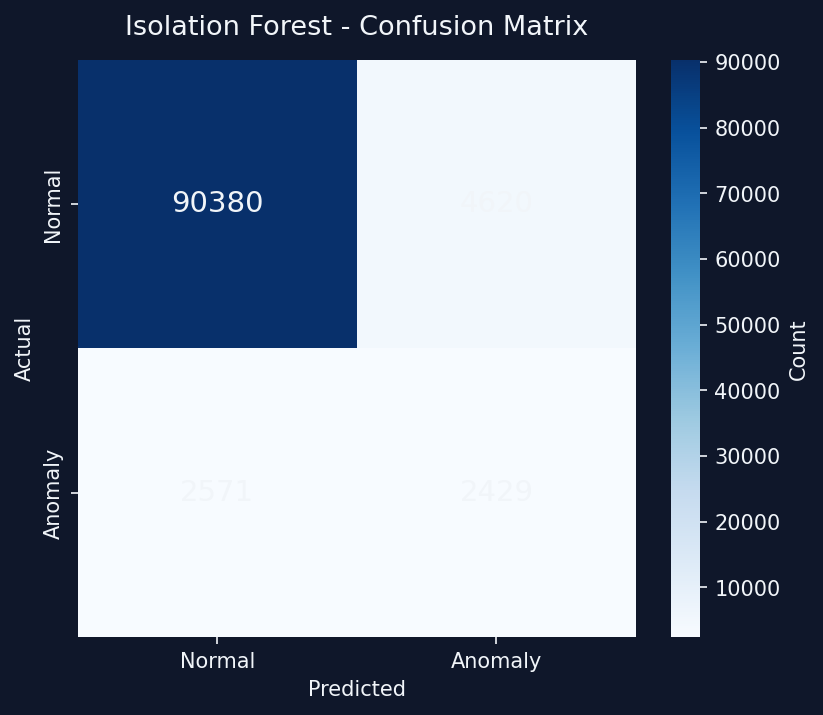
\includegraphics[width=0.31\textwidth]{if_cm}}
\subfigure[K-Means]{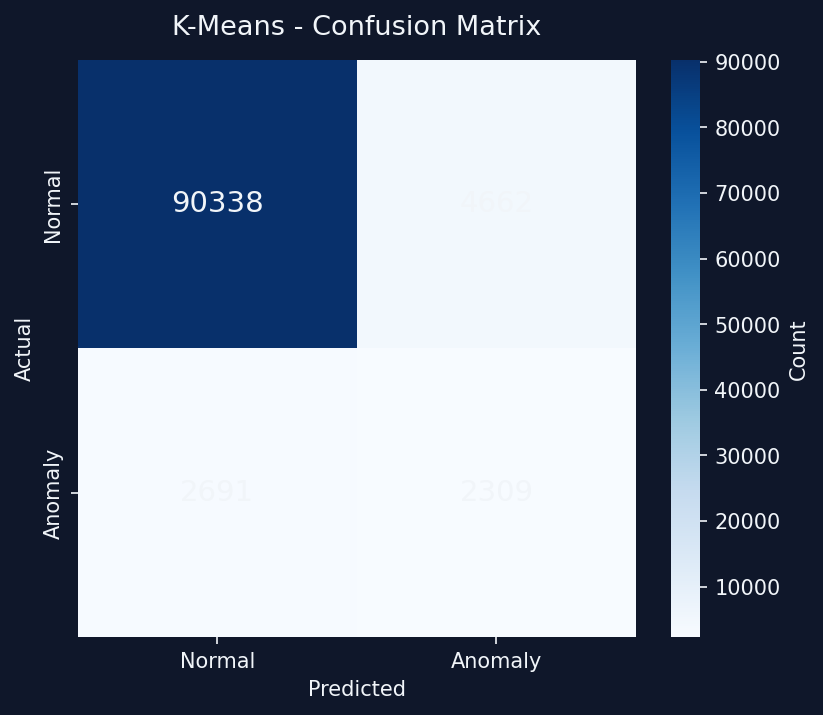
\includegraphics[width=0.31\textwidth]{km_cm}}
\subfigure[One-Class SVM]{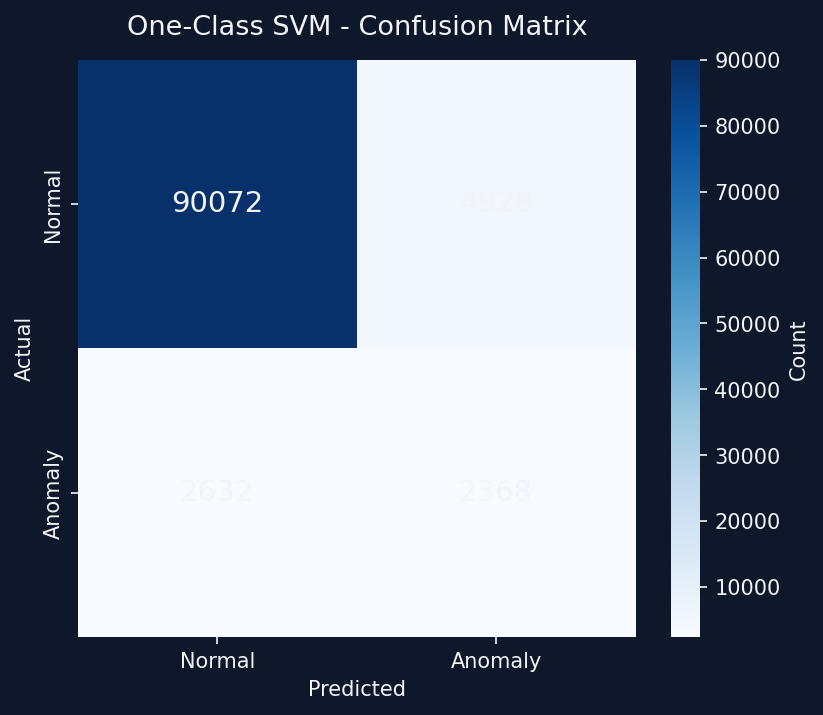
\includegraphics[width=0.31\textwidth]{oc_cm}}
\caption{Confusion Matrices for the three evaluated models.}
\label{fig:confusion_matrices}
\end{figure}

\section{Visual Model Comparison}
A visual comparison of the F1-scores and processing efficiencies was conducted to determine the best model for real-time industrial deployment.

\begin{figure}[!ht]
\centering
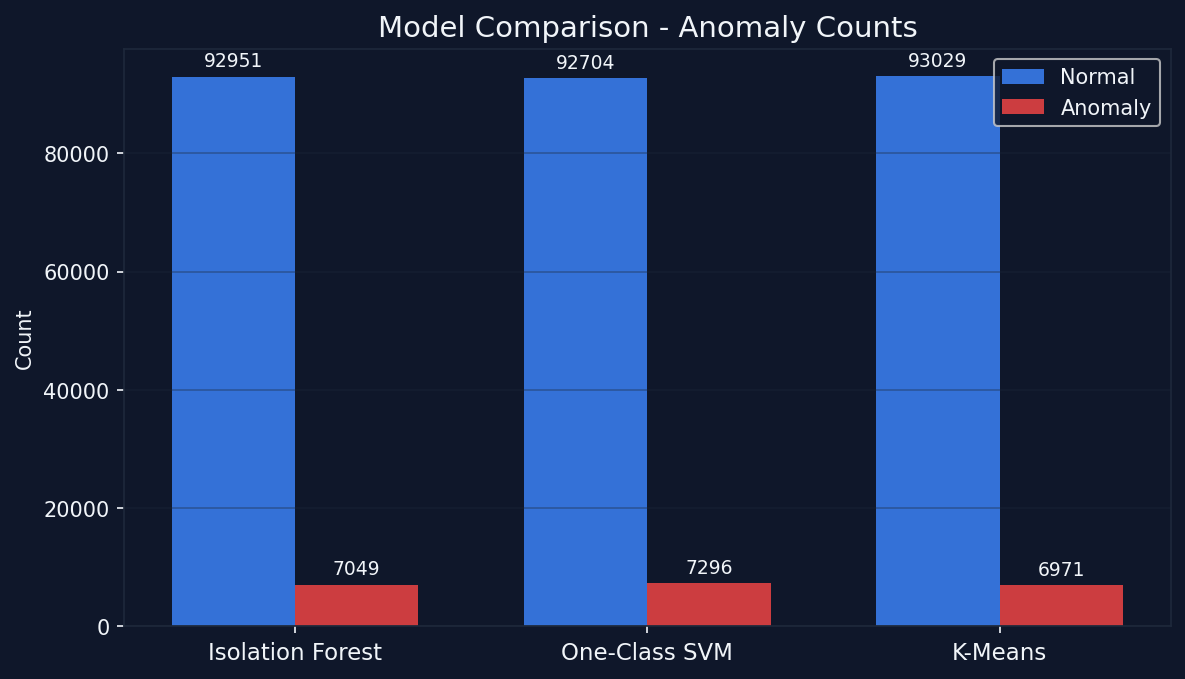
\includegraphics[width=0.8\textwidth]{model_comp_chart}
\caption{Comparative analysis of model performance metrics.}
\label{fig:model_comparison_chart}
\end{figure}

\section{Detailed Visual Diagnostic Analysis}
To further validate the model's performance, advanced diagnostic charts were generated for the \textbf{Isolation Forest} model, which demonstrated the most balanced results.

\subsection{Time-Series Anomaly Detection}
The time-series plot in Figure \ref{fig:if_timeseries} illustrates how the system flags anomalies in the \texttt{LogFloatValue} stream. The red markers indicate points that deviate significantly from the learned normal distribution.

\begin{figure}[!ht]
\centering
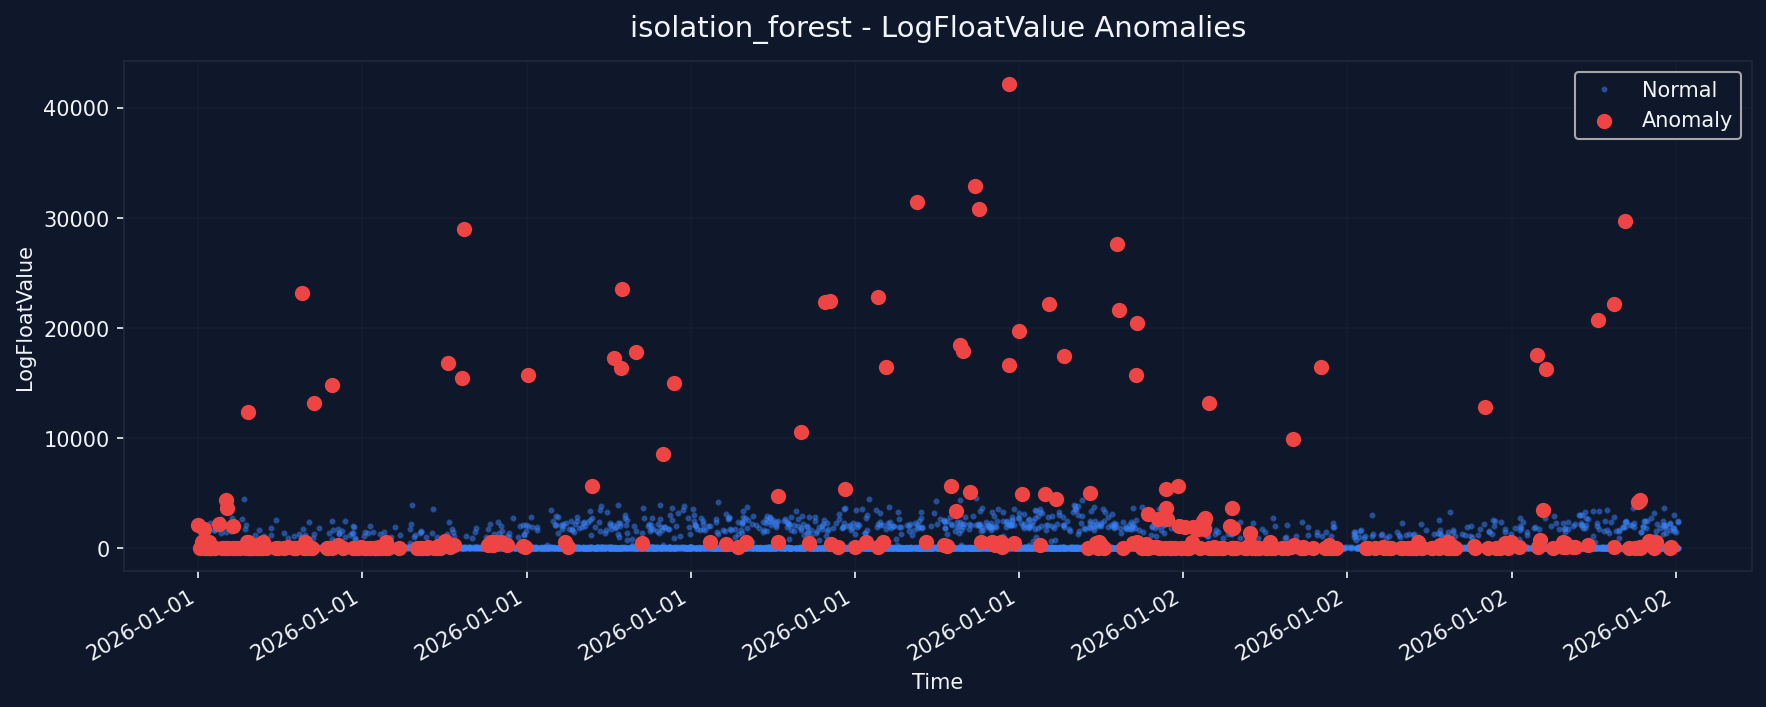
\includegraphics[width=0.95\textwidth]{if_timeseries}
\caption{Isolation Forest: Time-series visualization of detected anomalies in sensor signal.}
\label{fig:if_timeseries}
\end{figure}

\subsection{Anomaly Score Distribution}
The distribution of anomaly scores (Figure \ref{fig:if_scores}) reveals a clear decision boundary. Points with a score below zero are classified as anomalies, while the majority of the data clusters in the positive range, representing stable system behavior.

\begin{figure}[!ht]
\centering
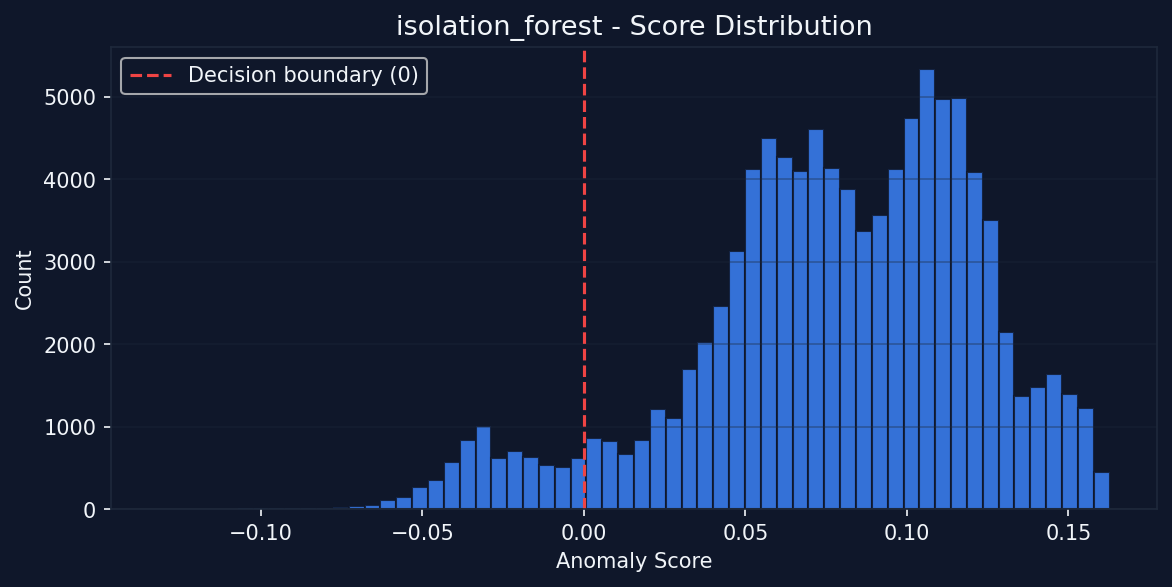
\includegraphics[width=0.8\textwidth]{if_scores}
\caption{Distribution of Anomaly Scores for Isolation Forest.}
\label{fig:if_scores}
\end{figure}

\subsection{Feature Interaction and Clustering}
The scatter plot in Figure \ref{fig:if_scatter} shows the interaction between \texttt{LogFloatValue} and \texttt{time\_delay\_sec}. It is evident that anomalies are not just extreme values, but often occur at specific combinations of signal level and network latency.

\begin{figure}[!ht]
\centering
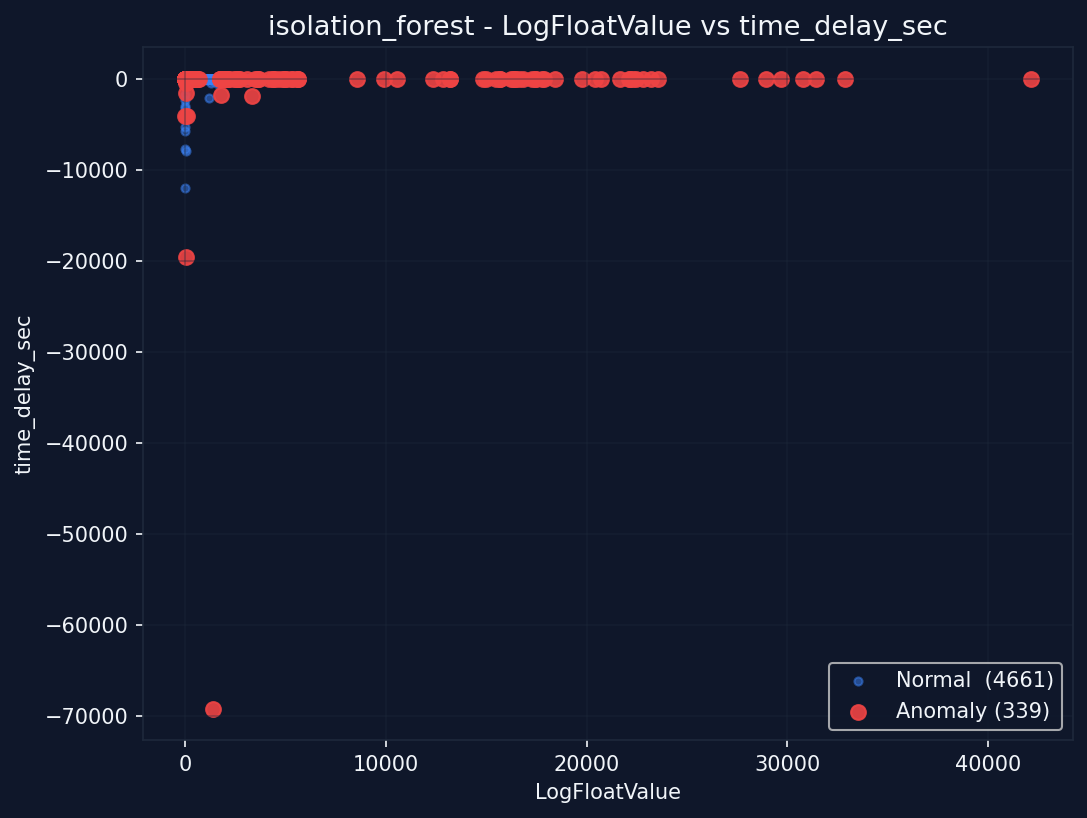
\includegraphics[width=0.8\textwidth]{if_scatter}
\caption{2D Scatter Plot: Interaction between sensor signal and network delay.}
\label{fig:if_scatter}
\end{figure}

The source code for the entire machine learning pipeline and the evaluation logic is available in the project repository \cite{iot_anomaly_source}.


Isolation Forest was found to be the most efficient for large batches, while One-Class SVM was better at finding anomalies in data with more complex distributions.

\section{Case Study: Network Delay and Outliers}
In the testing phase, several records were flagged as anomalies not because of extreme sensor values, but because of high ``Net Delay.'' For instance, records with a delay of over 120 seconds were visually flagged in red on the dashboard. This allowed the system to identify potential gateway hardware issues that a standard sensor-value monitor would have missed.

Furthermore, the IQR flagging successfully identified records where the \texttt{LogFloatValue} was physically possible but statistically improbable for that specific sensor type, adding an extra layer of validation before the machine learning phase.

\section{Dashboard Utility}
The implementation of the professional dashboard significantly improved the usability of the results. Key features like the \textbf{Device ID badge} and the \textbf{Excel Export} allowed for:
\begin{enumerate}
    \item \textbf{Traceability}: Quickly identifying which station (\texttt{RmsStationId}) was failing.
    \item \textbf{Offline Analysis}: Exporting filtered anomaly lists into \texttt{.xlsx} format for management reporting.
    \item \textbf{Visual Alerts}: The use of color-coded badges (Green/Amber/Red) allowed for ``at-a-glance'' status monitoring of network health.
\end{enumerate}

\section{Visual Comparative Analysis}
The ``Model Comparison Dashboard'' serves as a powerful research tool by providing a side-by-side metric breakdown (Anomaly Count, Percentage, and Average Score) across all algorithms. 

\begin{figure}[!ht]
\centering
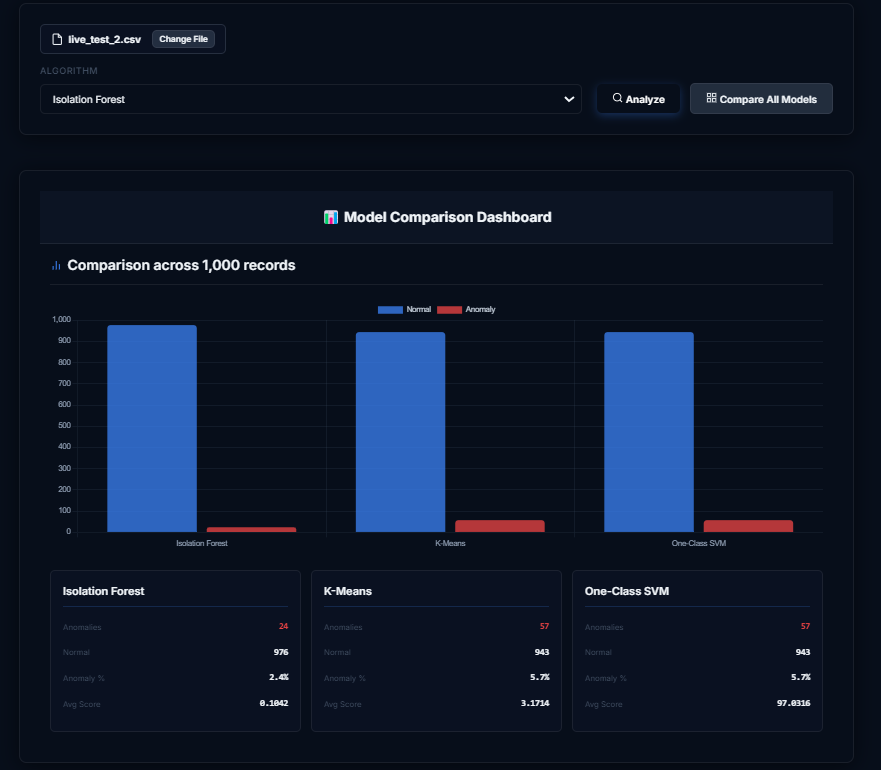
\includegraphics[width=0.9\textwidth]{compare_model_dashboard.png}
\caption{Model Comparison Dashboard showing the side-by-side distribution of anomalies across all evaluated algorithms.}
\label{fig:compare_dashboard}
\end{figure}

During testing, this visualization revealed that different algorithms exhibited varying levels of ``strictness.'' For example, K-Means often flagged more anomalies in high-noise datasets, while Isolation Forest was more effective at detecting isolated spikes in low-noise environments. This visual feedback was instrumental in validating the theoretical performance metrics presented earlier in this chapter.

\section{System Robustness and Diagnostic Warnings}
A critical aspect of the implemented system is its multi-layered validation. In addition to the ML predictions, the system provides several automated diagnostic warnings:
\begin{itemize}
    \item \textbf{Network Latency (Net Delay)}: The system identifies records with high latency ($>30s$) and flags them with a red badge, allowing operators to distinguish between sensor anomalies and network congestion.
    \item \textbf{Future Timestamp Detection}: A clock icon is displayed for records with a \texttt{LogTime} in the future relative to the \texttt{ServerTime}, indicating potential device clock synchronization issues.
    \item \textbf{Statistical Outliers (IQR)}: Even if the ML model classifies a point as "Normal," the system may flag it as a statistical outlier based on IQR analysis, providing a second opinion to the operator.
\end{itemize}
\begin{figure}[!ht]
\centering
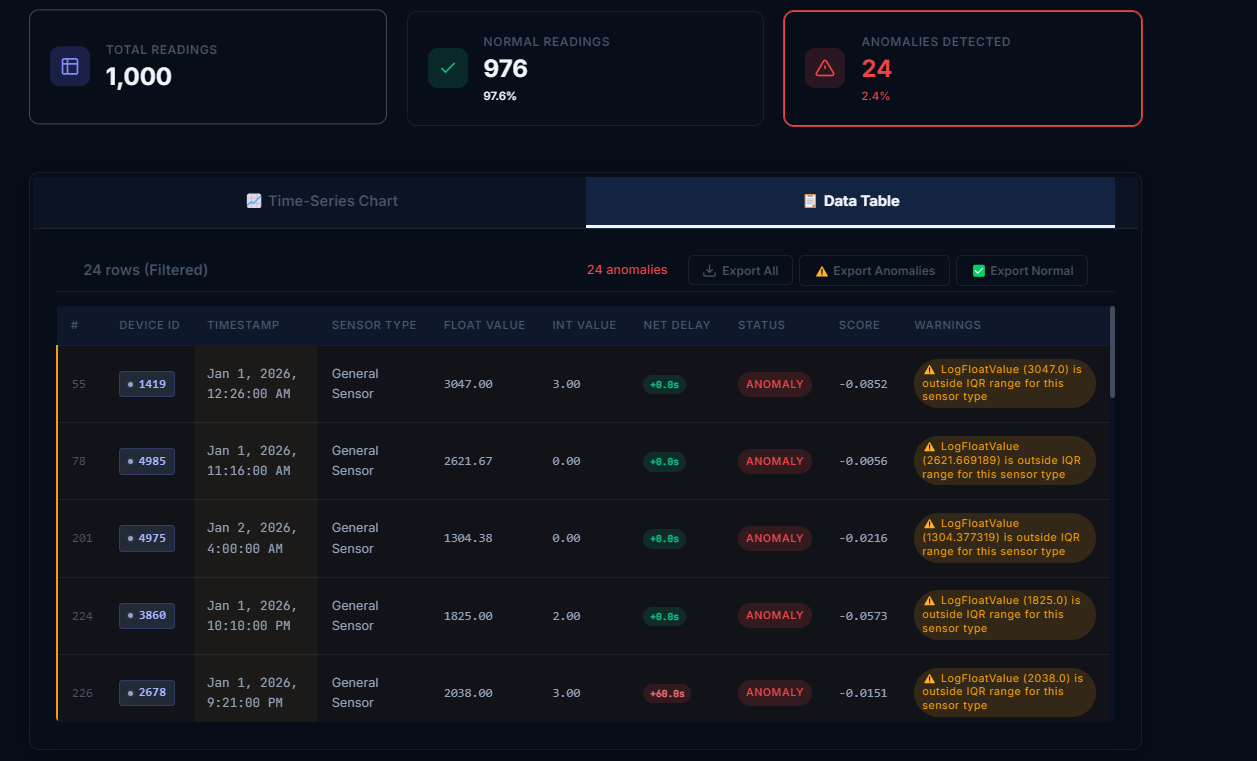
\includegraphics[width=0.9\textwidth]{data_table_net_time.png}
\caption{Detailed diagnostic view showing automated warnings for statistical outliers (IQR) and high network latency within the filtered anomaly table.}
\label{fig:data_table_warnings}
\end{figure}

This combination of unsupervised machine learning and rule-based diagnostic alerts makes the system highly robust for industrial environments.


\begin{figure}[!ht]
\centering
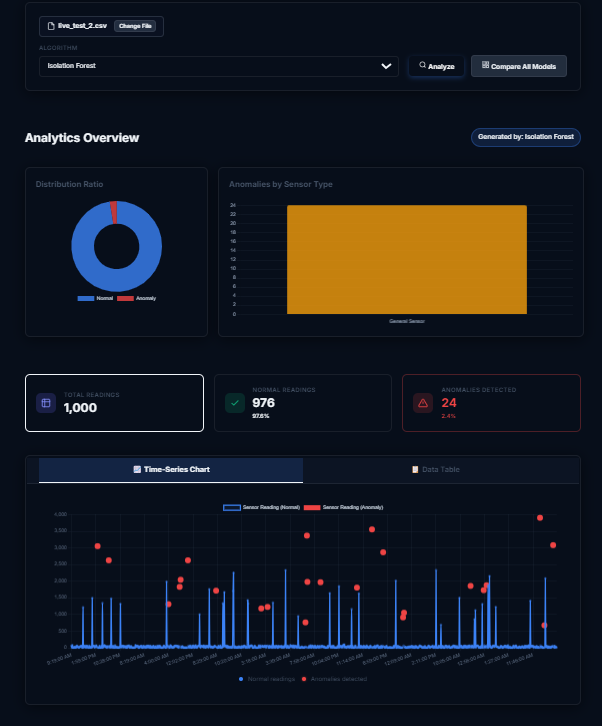
\includegraphics[width=0.9\textwidth]{dashboard.png}
\caption{The integrated IoT Anomaly Detection Dashboard showing the single-model analysis view with distribution charts and time-series trends.}
\label{fig:dashboard}
\end{figure}
